\documentclass[aspectratio=169]{beamer}
\usepackage{amsmath}
\usepackage{amssymb}
\usepackage{tikz}
\usepackage{xcolor}
\usetikzlibrary{shapes,backgrounds,patterns}

\usepackage{pgfplots}
\pgfplotsset{compat=1.18, legend cell align=left}
\usetikzlibrary{arrows.meta,decorations.pathreplacing,calc,positioning}
\usepackage{booktabs}

% royalblue isn't a base xcolor name, so define it first (this is the default accent)
\definecolor{royalblue}{RGB}{65,105,225}

% ============================================================
%  ACCENT COLOR: change ONE line below to switch the theme
%  Choose one of: royalblue , red , black
% ============================================================
\colorlet{accent}{royalblue}
% \colorlet{accent}{red}
% \colorlet{accent}{black}
% ============================================================

% colorblind-safe, high-contrast second color (Okabe-Ito vermillion)
\definecolor{hl}{RGB}{213,94,0}

\usetheme{default}
\setbeamercolor{background canvas}{bg=white}
\setbeamercolor{normal text}{fg=black}
\setbeamercolor{structure}{fg=accent}
\setbeamercolor{frametitle}{fg=accent,bg=white}
\setbeamercolor{title}{fg=accent}
\setbeamercolor{section in toc}{fg=black}
\setbeamercolor{block title}{fg=black,bg=gray!10}
\setbeamercolor{block body}{fg=black,bg=gray!5}
\setbeamercolor{block title example}{fg=black,bg=green!10}
\setbeamercolor{block body example}{fg=black,bg=green!5}
\setbeamercolor{block title alerted}{fg=black,bg=red!10}
\setbeamercolor{block body alerted}{fg=black,bg=red!5}

\setbeamertemplate{navigation symbols}{}
\setbeamertemplate{footline}{
    \hfill\makebox[5pt]{%
        \scriptsize\insertframenumber}
    \hspace*{2em}
    \vspace{0.5cm}
}

\newcommand{\cbox}[2]{\colorbox{#1}{\ensuremath{\displaystyle #2}}}

\pgfplotsset{
  miniplot/.style={
    width=4.0cm, height=3.0cm,
    axis lines=middle, xtick=\empty, ytick=\empty,
    samples=120, thick, clip=true
  }
}

\title{Interpolation: The Ideas Behind the Code}
\subtitle{Lines, polynomials, splines, and shape preservation}
\author{Sharareh Sayyad}
\institute{Washington State University}
\date{\today}


\begin{document}

\frame{\titlepage}

% ============================================================
% 0. Why interpolation
% ============================================================
\begin{frame}{Why do we need interpolation?}
\begin{columns}[c]
\begin{column}{0.46\textwidth}
\small
We often know a quantity \textbf{only at a few points}, but need it \textbf{in between}.
\vspace{0.1cm}
\begin{itemize}
  \setlength{\itemsep}{3pt}
  \item \textbf{Measurements:} a sensor reads once per hour.
  \item \textbf{Tables:} e.g.\ steam tables.
  \item \textbf{Expensive functions:} hours of computing per point.
  \item \textbf{Other methods:} integration, derivatives, ODE solvers build on it.
\end{itemize}
\vspace{0.1cm}
\begin{block}{The task}
\[
\text{given } (x_i, y_i), \text{ find } p \text{ with } \cbox{accent!12}{p(x_i) = y_i}
\]
\end{block}
\end{column}
\begin{column}{0.52\textwidth}
\centering
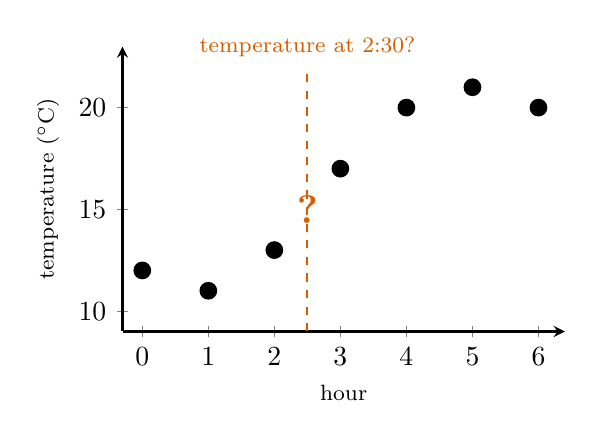
\begin{tikzpicture}
\begin{axis}[width=7.2cm, height=5.2cm, axis lines=left, xmin=-0.3, xmax=6.4, ymin=9, ymax=23,
  xtick={0,...,6}, ytick={10,15,20}, thick, clip=false,
  xlabel={hour}, ylabel={temperature ($^\circ$C)}, label style={font=\footnotesize}]
  \addplot[black, only marks, mark=*, mark size=2.8pt] coordinates {(0.0000,12.0000) (1.0000,11.0000) (2.0000,13.0000) (3.0000,17.0000) (4.0000,20.0000) (5.0000,21.0000) (6.0000,20.0000)};
  \draw[hl, dashed, thick] (axis cs:2.5,9) -- (axis cs:2.5,22);
  \node[hl, font=\Large\bfseries] at (axis cs:2.5,15) {?};
  \node[hl, font=\footnotesize, anchor=south] at (axis cs:2.5,22) {temperature at 2:30?};
\end{axis}
\end{tikzpicture}\\[2pt]
\footnotesize Hourly readings. What was the temperature at 2:30?\\
The answer depends on \textbf{how we connect the dots}: that is this lecture.
\end{column}
\end{columns}
\end{frame}

% ============================================================
% 1. Straight-line interpolation
% ============================================================
\begin{frame}{Idea 1: connect the dots with straight lines}
\begin{columns}[c]
\begin{column}{0.46\textwidth}
\small
On each interval $[x_i, x_{i+1}]$:
\[
\cbox{accent!12}{p(x) = (1-t)\,y_i + t\,y_{i+1}}
\]
\[
t = \frac{x - x_i}{x_{i+1} - x_i} \in [0, 1]
\]
A \textbf{weighted average} of the two neighbours.
\vspace{0.2cm}
\begin{exampleblock}{Good}
\footnotesize
Local: only 2 points matter. Never overshoots.\\
Error $\le \tfrac{h^2}{8}\max|f''|$: halve $h$, error $\div 4$.
\end{exampleblock}
\begin{alertblock}{Not so good}
\footnotesize
A \textbf{corner} at every node.
\end{alertblock}
\end{column}
\begin{column}{0.52\textwidth}
\centering
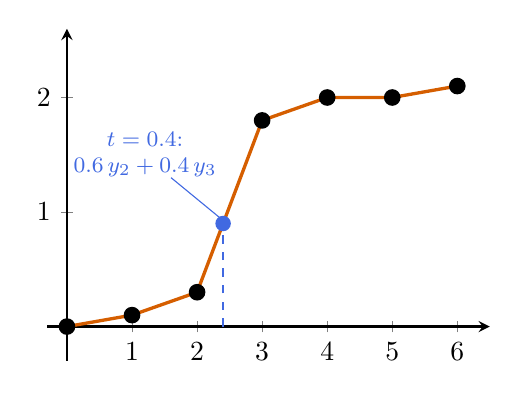
\begin{tikzpicture}
\begin{axis}[width=7.2cm, height=5.8cm, axis lines=middle, xmin=-0.3, xmax=6.5, ymin=-0.3, ymax=2.6,
  xtick={0,...,6}, ytick={1,2}, thick, clip=false]
  \addplot[hl, very thick] coordinates {(0.0000,0.0000) (1.0000,0.1000) (2.0000,0.3000) (3.0000,1.8000) (4.0000,2.0000) (5.0000,2.0000) (6.0000,2.1000)};
  \addplot[black, only marks, mark=*, mark size=2.6pt] coordinates {(0.0000,0.0000) (1.0000,0.1000) (2.0000,0.3000) (3.0000,1.8000) (4.0000,2.0000) (5.0000,2.0000) (6.0000,2.1000)};
  \draw[accent, dashed, thick] (axis cs:2.4,0) -- (axis cs:2.4,0.9);
  \fill[accent] (axis cs:2.4,0.9) circle (2.8pt);
  \node[accent, font=\footnotesize, align=center] at (axis cs:1.2,1.5) {$t = 0.4$:\\$0.6\,y_2 + 0.4\,y_3$};
  \draw[accent, thin] (axis cs:1.6,1.3) -- (axis cs:2.35,0.95);
\end{axis}
\end{tikzpicture}\\[2pt]
\footnotesize \textbf{Running example:} 7 points that rise, then level off.\\
We use the same data for every method.
\end{column}
\end{columns}
\end{frame}

% ============================================================
% 2. Global polynomial
% ============================================================
\begin{frame}{Idea 2: one polynomial through all the points}
\begin{columns}[c]
\begin{column}{0.46\textwidth}
\small
\begin{block}{Degree $n$ $\Rightarrow$ $n+1$ coefficients}
\footnotesize
\setlength{\tabcolsep}{3pt}
\begin{tabular}{llcc}
 & & \textbf{deg.} & \textbf{coeff.} \\
line & $a + bx$ & 1 & 2 \\
quadratic & $a + bx + cx^2$ & 2 & 3 \\
cubic & $a + bx + cx^2 + dx^3$ & 3 & 4 \\
\end{tabular}\\[3pt]
Each coefficient lets us hit one more point:\\
$n+1$ points $\Rightarrow$ one polynomial of degree $n$.
\end{block}
\footnotesize \textbf{Good:} one formula, smooth everywhere, no corners.
\begin{alertblock}{Not so good: it is global}
\footnotesize
Every point affects the \textbf{whole} curve.\\
To bend at $x = 3$, it must \textbf{wiggle} elsewhere.
\end{alertblock}

\end{column}
\begin{column}{0.52\textwidth}
\centering
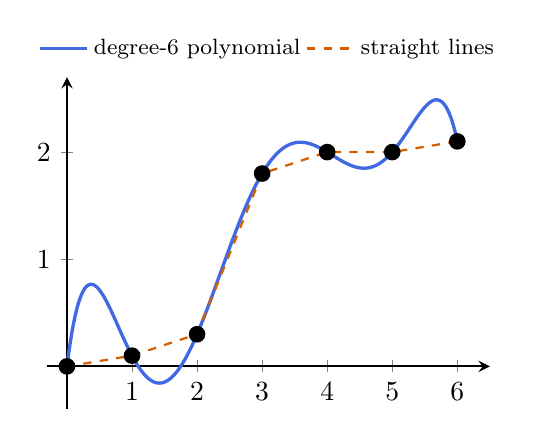
\begin{tikzpicture}
\begin{axis}[width=7.2cm, height=5.8cm, axis lines=middle, xmin=-0.3, xmax=6.5, ymin=-0.4, ymax=2.7,
  xtick={0,...,6}, ytick={1,2}, thick, clip=false,
  legend style={font=\footnotesize, at={(0.5,1.02)}, anchor=south, draw=none}, legend columns=2]
  \addplot[accent, very thick] coordinates {(0.0000,-0.0000) (0.0250,0.1164) (0.0500,0.2209) (0.0750,0.3143) (0.1000,0.3970) (0.1250,0.4698) (0.1500,0.5332) (0.1750,0.5877) (0.2000,0.6339) (0.2250,0.6724) (0.2500,0.7035) (0.2750,0.7278) (0.3000,0.7458) (0.3250,0.7579) (0.3500,0.7645) (0.3750,0.7661) (0.4000,0.7631) (0.4250,0.7558) (0.4500,0.7446) (0.4750,0.7300) (0.5000,0.7121) (0.5250,0.6914) (0.5500,0.6682) (0.5750,0.6427) (0.6000,0.6153) (0.6250,0.5862) (0.6500,0.5557) (0.6750,0.5241) (0.7000,0.4915) (0.7250,0.4583) (0.7500,0.4245) (0.7750,0.3905) (0.8000,0.3564) (0.8250,0.3224) (0.8500,0.2886) (0.8750,0.2553) (0.9000,0.2225) (0.9250,0.1905) (0.9500,0.1593) (0.9750,0.1291) (1.0000,0.1000) (1.0250,0.0721) (1.0500,0.0454) (1.0750,0.0202) (1.1000,-0.0036) (1.1250,-0.0259) (1.1500,-0.0466) (1.1750,-0.0656) (1.2000,-0.0829) (1.2250,-0.0984) (1.2500,-0.1122) (1.2750,-0.1241) (1.3000,-0.1342) (1.3250,-0.1424) (1.3500,-0.1487) (1.3750,-0.1531) (1.4000,-0.1555) (1.4250,-0.1561) (1.4500,-0.1548) (1.4750,-0.1516) (1.5000,-0.1465) (1.5250,-0.1395) (1.5500,-0.1307) (1.5750,-0.1201) (1.6000,-0.1077) (1.6250,-0.0935) (1.6500,-0.0776) (1.6750,-0.0600) (1.7000,-0.0408) (1.7250,-0.0200) (1.7500,0.0024) (1.7750,0.0263) (1.8000,0.0516) (1.8250,0.0783) (1.8500,0.1064) (1.8750,0.1358) (1.9000,0.1664) (1.9250,0.1982) (1.9500,0.2311) (1.9750,0.2651) (2.0000,0.3000) (2.0250,0.3359) (2.0500,0.3726) (2.0750,0.4101) (2.1000,0.4484) (2.1250,0.4873) (2.1500,0.5269) (2.1750,0.5669) (2.2000,0.6075) (2.2250,0.6484) (2.2500,0.6897) (2.2750,0.7313) (2.3000,0.7731) (2.3250,0.8150) (2.3500,0.8570) (2.3750,0.8990) (2.4000,0.9410) (2.4250,0.9829) (2.4500,1.0247) (2.4750,1.0662) (2.5000,1.1074) (2.5250,1.1483) (2.5500,1.1889) (2.5750,1.2290) (2.6000,1.2686) (2.6250,1.3076) (2.6500,1.3461) (2.6750,1.3839) (2.7000,1.4211) (2.7250,1.4575) (2.7500,1.4932) (2.7750,1.5280) (2.8000,1.5620) (2.8250,1.5952) (2.8500,1.6274) (2.8750,1.6587) (2.9000,1.6890) (2.9250,1.7183) (2.9500,1.7466) (2.9750,1.7738) (3.0000,1.8000) (3.0250,1.8251) (3.0500,1.8491) (3.0750,1.8719) (3.1000,1.8936) (3.1250,1.9142) (3.1500,1.9336) (3.1750,1.9519) (3.2000,1.9690) (3.2250,1.9850) (3.2500,1.9998) (3.2750,2.0135) (3.3000,2.0260) (3.3250,2.0374) (3.3500,2.0476) (3.3750,2.0568) (3.4000,2.0648) (3.4250,2.0718) (3.4500,2.0777) (3.4750,2.0825) (3.5000,2.0863) (3.5250,2.0892) (3.5500,2.0910) (3.5750,2.0920) (3.6000,2.0920) (3.6250,2.0911) (3.6500,2.0894) (3.6750,2.0869) (3.7000,2.0836) (3.7250,2.0796) (3.7500,2.0750) (3.7750,2.0696) (3.8000,2.0637) (3.8250,2.0572) (3.8500,2.0502) (3.8750,2.0427) (3.9000,2.0348) (3.9250,2.0265) (3.9500,2.0179) (3.9750,2.0091) (4.0000,2.0000) (4.0250,1.9908) (4.0500,1.9814) (4.0750,1.9720) (4.1000,1.9626) (4.1250,1.9532) (4.1500,1.9439) (4.1750,1.9348) (4.2000,1.9258) (4.2250,1.9171) (4.2500,1.9088) (4.2750,1.9007) (4.3000,1.8931) (4.3250,1.8860) (4.3500,1.8794) (4.3750,1.8733) (4.4000,1.8678) (4.4250,1.8629) (4.4500,1.8588) (4.4750,1.8554) (4.5000,1.8527) (4.5250,1.8509) (4.5500,1.8499) (4.5750,1.8498) (4.6000,1.8506) (4.6250,1.8523) (4.6500,1.8550) (4.6750,1.8587) (4.7000,1.8634) (4.7250,1.8691) (4.7500,1.8759) (4.7750,1.8837) (4.8000,1.8925) (4.8250,1.9024) (4.8500,1.9133) (4.8750,1.9253) (4.9000,1.9383) (4.9250,1.9523) (4.9500,1.9672) (4.9750,1.9832) (5.0000,2.0000) (5.0250,2.0177) (5.0500,2.0363) (5.0750,2.0556) (5.1000,2.0757) (5.1250,2.0964) (5.1500,2.1177) (5.1750,2.1395) (5.2000,2.1618) (5.2250,2.1844) (5.2500,2.2072) (5.2750,2.2301) (5.3000,2.2530) (5.3250,2.2758) (5.3500,2.2983) (5.3750,2.3204) (5.4000,2.3420) (5.4250,2.3628) (5.4500,2.3827) (5.4750,2.4016) (5.5000,2.4191) (5.5250,2.4352) (5.5500,2.4496) (5.5750,2.4621) (5.6000,2.4724) (5.6250,2.4803) (5.6500,2.4856) (5.6750,2.4878) (5.7000,2.4869) (5.7250,2.4824) (5.7500,2.4741) (5.7750,2.4616) (5.8000,2.4445) (5.8250,2.4226) (5.8500,2.3955) (5.8750,2.3627) (5.9000,2.3239) (5.9250,2.2787) (5.9500,2.2266) (5.9750,2.1672) (6.0000,2.1000)};
  \addlegendentry{degree-6 polynomial}
  \addplot[hl, thick, dashed] coordinates {(0.0000,0.0000) (1.0000,0.1000) (2.0000,0.3000) (3.0000,1.8000) (4.0000,2.0000) (5.0000,2.0000) (6.0000,2.1000)};
  \addlegendentry{straight lines}
  \addplot[black, only marks, mark=*, mark size=2.6pt] coordinates {(0.0000,0.0000) (1.0000,0.1000) (2.0000,0.3000) (3.0000,1.8000) (4.0000,2.0000) (5.0000,2.0000) (6.0000,2.1000)};
\end{axis}
\end{tikzpicture}\\[2pt]
\footnotesize Smooth, but it bulges above the last points and dips below zero.
\end{column}
\end{columns}
\end{frame}

% ============================================================
% 3. Piecewise idea
% ============================================================
\begin{frame}{Idea 3: piecewise polynomials}
\begin{columns}[c]
\begin{column}{0.46\textwidth}
\small
Use a \textbf{separate cubic on each interval}.
\vspace{0.2cm}
\begin{itemize}
  \setlength{\itemsep}{5pt}
  \item \textbf{Local} like straight lines.
  \item \textbf{Smooth} like polynomials.
\end{itemize}
\vspace{0.2cm}
\begin{block}{A cubic (degree 3) has 4 coefficients}
\footnotesize
So each piece can meet 4 conditions:\\[4pt]
\textbf{2 values} $y_i,\ y_{i+1}$ \quad $\leftarrow$ given by the data\\[2pt]
\textbf{2 slopes} $d_i,\ d_{i+1}$ \quad $\leftarrow$ \textcolor{accent}{\textbf{we choose}}
\end{block}
\vspace{0.1cm}
\begin{exampleblock}{The big idea}
\footnotesize
Different cubic methods = \textbf{different rules for choosing the slopes $d_i$}.
\end{exampleblock}
\end{column}
\begin{column}{0.52\textwidth}
\centering
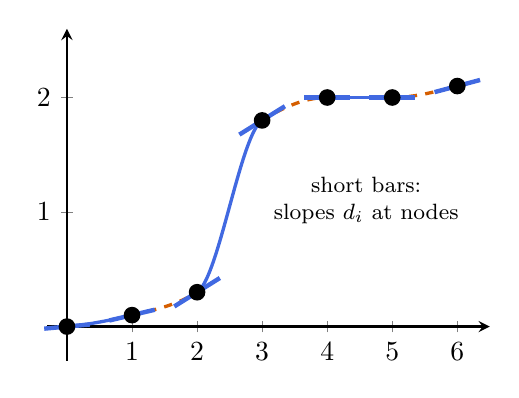
\begin{tikzpicture}
\begin{axis}[width=7.2cm, height=5.8cm, axis lines=middle, xmin=-0.3, xmax=6.5, ymin=-0.3, ymax=2.6,
  xtick={0,...,6}, ytick={1,2}, thick, clip=false]
  \addplot[accent, very thick] coordinates {(0.0000,0.0000) (0.0250,0.0013) (0.0500,0.0027) (0.0750,0.0041) (0.1000,0.0057) (0.1250,0.0073) (0.1500,0.0089) (0.1750,0.0107) (0.2000,0.0125) (0.2250,0.0144) (0.2500,0.0164) (0.2750,0.0184) (0.3000,0.0206) (0.3250,0.0227) (0.3500,0.0250) (0.3750,0.0272) (0.4000,0.0296) (0.4250,0.0320) (0.4500,0.0345) (0.4750,0.0370) (0.5000,0.0396) (0.5250,0.0422) (0.5500,0.0449) (0.5750,0.0476) (0.6000,0.0504) (0.6250,0.0532) (0.6500,0.0561) (0.6750,0.0590) (0.7000,0.0620) (0.7250,0.0649) (0.7500,0.0680) (0.7750,0.0710) (0.8000,0.0741) (0.8250,0.0773) (0.8500,0.0804) (0.8750,0.0836) (0.9000,0.0869) (0.9250,0.0901) (0.9500,0.0934) (0.9750,0.0967) (1.0000,0.1000)};
  \addplot[hl, very thick, dashed] coordinates {(1.0000,0.1000) (1.0250,0.1033) (1.0500,0.1066) (1.0750,0.1099) (1.1000,0.1132) (1.1250,0.1165) (1.1500,0.1198) (1.1750,0.1232) (1.2000,0.1266) (1.2250,0.1300) (1.2500,0.1335) (1.2750,0.1370) (1.3000,0.1406) (1.3250,0.1442) (1.3500,0.1480) (1.3750,0.1518) (1.4000,0.1557) (1.4250,0.1597) (1.4500,0.1639) (1.4750,0.1682) (1.5000,0.1725) (1.5250,0.1771) (1.5500,0.1818) (1.5750,0.1866) (1.6000,0.1916) (1.6250,0.1967) (1.6500,0.2021) (1.6750,0.2076) (1.7000,0.2133) (1.7250,0.2192) (1.7500,0.2254) (1.7750,0.2317) (1.8000,0.2383) (1.8250,0.2451) (1.8500,0.2521) (1.8750,0.2595) (1.9000,0.2670) (1.9250,0.2748) (1.9500,0.2829) (1.9750,0.2913) (2.0000,0.3000)};
  \addplot[accent, very thick] coordinates {(2.0000,0.3000) (2.0250,0.3109) (2.0500,0.3260) (2.0750,0.3449) (2.1000,0.3674) (2.1250,0.3934) (2.1500,0.4226) (2.1750,0.4549) (2.2000,0.4899) (2.2250,0.5275) (2.2500,0.5675) (2.2750,0.6096) (2.3000,0.6536) (2.3250,0.6994) (2.3500,0.7467) (2.3750,0.7953) (2.4000,0.8449) (2.4250,0.8955) (2.4500,0.9466) (2.4750,0.9982) (2.5000,1.0500) (2.5250,1.1018) (2.5500,1.1534) (2.5750,1.2045) (2.6000,1.2551) (2.6250,1.3047) (2.6500,1.3533) (2.6750,1.4006) (2.7000,1.4464) (2.7250,1.4904) (2.7500,1.5325) (2.7750,1.5725) (2.8000,1.6101) (2.8250,1.6451) (2.8500,1.6774) (2.8750,1.7066) (2.9000,1.7326) (2.9250,1.7551) (2.9500,1.7740) (2.9750,1.7891) (3.0000,1.8000)};
  \addplot[hl, very thick, dashed] coordinates {(3.0000,1.8000) (3.0250,1.8088) (3.0500,1.8174) (3.0750,1.8259) (3.1000,1.8342) (3.1250,1.8424) (3.1500,1.8504) (3.1750,1.8583) (3.2000,1.8660) (3.2250,1.8735) (3.2500,1.8809) (3.2750,1.8881) (3.3000,1.8951) (3.3250,1.9019) (3.3500,1.9085) (3.3750,1.9150) (3.4000,1.9212) (3.4250,1.9273) (3.4500,1.9331) (3.4750,1.9387) (3.5000,1.9441) (3.5250,1.9493) (3.5500,1.9543) (3.5750,1.9590) (3.6000,1.9635) (3.6250,1.9677) (3.6500,1.9718) (3.6750,1.9755) (3.7000,1.9790) (3.7250,1.9823) (3.7500,1.9853) (3.7750,1.9880) (3.8000,1.9905) (3.8250,1.9927) (3.8500,1.9946) (3.8750,1.9962) (3.9000,1.9976) (3.9250,1.9986) (3.9500,1.9994) (3.9750,1.9998) (4.0000,2.0000)};
  \addplot[accent, very thick] coordinates {(4.0000,2.0000) (4.0250,2.0000) (4.0500,2.0000) (4.0750,2.0000) (4.1000,2.0000) (4.1250,2.0000) (4.1500,2.0000) (4.1750,2.0000) (4.2000,2.0000) (4.2250,2.0000) (4.2500,2.0000) (4.2750,2.0000) (4.3000,2.0000) (4.3250,2.0000) (4.3500,2.0000) (4.3750,2.0000) (4.4000,2.0000) (4.4250,2.0000) (4.4500,2.0000) (4.4750,2.0000) (4.5000,2.0000) (4.5250,2.0000) (4.5500,2.0000) (4.5750,2.0000) (4.6000,2.0000) (4.6250,2.0000) (4.6500,2.0000) (4.6750,2.0000) (4.7000,2.0000) (4.7250,2.0000) (4.7500,2.0000) (4.7750,2.0000) (4.8000,2.0000) (4.8250,2.0000) (4.8500,2.0000) (4.8750,2.0000) (4.9000,2.0000) (4.9250,2.0000) (4.9500,2.0000) (4.9750,2.0000) (5.0000,2.0000)};
  \addplot[hl, very thick, dashed] coordinates {(5.0000,2.0000) (5.0250,2.0001) (5.0500,2.0004) (5.0750,2.0008) (5.1000,2.0015) (5.1250,2.0022) (5.1500,2.0032) (5.1750,2.0043) (5.2000,2.0056) (5.2250,2.0070) (5.2500,2.0086) (5.2750,2.0103) (5.3000,2.0122) (5.3250,2.0141) (5.3500,2.0162) (5.3750,2.0185) (5.4000,2.0208) (5.4250,2.0233) (5.4500,2.0258) (5.4750,2.0285) (5.5000,2.0312) (5.5250,2.0341) (5.5500,2.0371) (5.5750,2.0401) (5.6000,2.0432) (5.6250,2.0464) (5.6500,2.0496) (5.6750,2.0530) (5.7000,2.0564) (5.7250,2.0598) (5.7500,2.0633) (5.7750,2.0668) (5.8000,2.0704) (5.8250,2.0740) (5.8500,2.0777) (5.8750,2.0813) (5.9000,2.0851) (5.9250,2.0888) (5.9500,2.0925) (5.9750,2.0963) (6.0000,2.1000)};
  \draw[accent, line width=1.6pt] (axis cs:-0.350,-0.018) -- (axis cs:0.350,0.018); \draw[accent, line width=1.6pt] (axis cs:0.650,0.053) -- (axis cs:1.350,0.147); \draw[accent, line width=1.6pt] (axis cs:1.650,0.176) -- (axis cs:2.350,0.424); \draw[accent, line width=1.6pt] (axis cs:2.650,1.676) -- (axis cs:3.350,1.924); \draw[accent, line width=1.6pt] (axis cs:3.650,2.000) -- (axis cs:4.350,2.000); \draw[accent, line width=1.6pt] (axis cs:4.650,2.000) -- (axis cs:5.350,2.000); \draw[accent, line width=1.6pt] (axis cs:5.650,2.047) -- (axis cs:6.350,2.153);

  \addplot[black, only marks, mark=*, mark size=2.6pt] coordinates {(0.0000,0.0000) (1.0000,0.1000) (2.0000,0.3000) (3.0000,1.8000) (4.0000,2.0000) (5.0000,2.0000) (6.0000,2.1000)};
  \node[font=\footnotesize, align=center] at (axis cs:4.6,1.1) {short bars:\\slopes $d_i$ at nodes};
\end{axis}
\end{tikzpicture}\\[2pt]
\footnotesize Six pieces, alternating solid/dashed.\\
Neighbours share the value \textbf{and} the slope at each node.
\end{column}
\end{columns}
\end{frame}

% ============================================================
% 4. Hermite building blocks
% ============================================================
\begin{frame}{Building one piece: 2 points + 2 slopes = 1 cubic}
\begin{columns}[c]
\begin{column}{0.46\textwidth}
\small
One interval $[0, 1]$, one cubic $p(x) = a + bx + cx^2 + dx^3$.\\[4pt]
We ask for 4 things:\\[2pt]
\footnotesize
\hspace*{1em}values: \ $p(0) = y_0$, \ $p(1) = y_1$\\
\hspace*{1em}slopes: \ $p'(0) = d_0$, \ $p'(1) = d_1$\\[2pt]
\begin{block}{Solving gives the 4 coefficients}
\footnotesize
$a = y_0, \qquad b = d_0$\\[3pt]
$c = 3(y_1 - y_0) - 2d_0 - d_1$\\[3pt]
$d = 2(y_0 - y_1) + d_0 + d_1$
\end{block}
\begin{exampleblock}{Message}
\footnotesize
Points: \textbf{fixed by the data}. Slopes: \textbf{our choice}, and they decide the shape.
\end{exampleblock}
\end{column}
\begin{column}{0.52\textwidth}
\centering
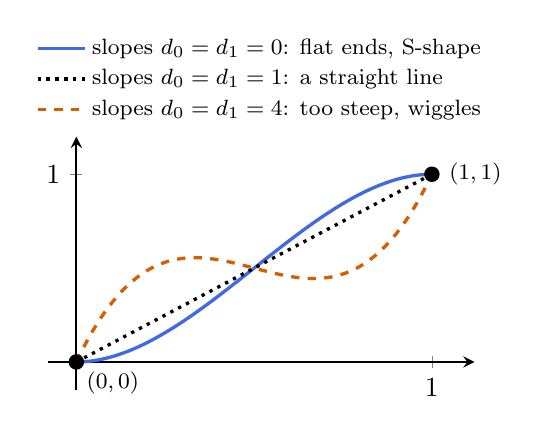
\begin{tikzpicture}
\begin{axis}[width=7.0cm, height=4.8cm, axis lines=middle, xmin=-0.08, xmax=1.12, ymin=-0.15, ymax=1.2,
  xtick={0,1}, ytick={1}, samples=100, thick, clip=false,
  legend style={font=\footnotesize, at={(0.5,1.02)}, anchor=south, draw=none}, legend columns=1]
  \addplot[accent, very thick, domain=0:1] {3*x^2-2*x^3};
  \addlegendentry{slopes $d_0 = d_1 = 0$: flat ends, S-shape}
  \addplot[black, very thick, dotted, domain=0:1] {x};
  \addlegendentry{slopes $d_0 = d_1 = 1$: a straight line}
  \addplot[hl, very thick, dashed, domain=0:1] {4*x-9*x^2+6*x^3};
  \addlegendentry{slopes $d_0 = d_1 = 4$: too steep, wiggles}
  \fill (axis cs:0,0) circle (2.8pt);
  \fill (axis cs:1,1) circle (2.8pt);
  \node[font=\footnotesize, below right] at (axis cs:0,0) {$(0, 0)$};
  \node[font=\footnotesize, right] at (axis cs:1.02,1) {$(1, 1)$};
\end{axis}
\end{tikzpicture}\\[2pt]
\footnotesize Same two points, three slope choices, three cubics.\\
Neighbours share the slope at a node $\Rightarrow$ no corners.
\end{column}
\end{columns}
\end{frame}

% ============================================================
% 5. Cubic spline
% ============================================================
\begin{frame}{Rule A, cubic spline: match the second derivative too}
\begin{columns}[c]
\begin{column}{0.49\textwidth}
\small
New requirement: \textbf{$p''$ continuous} at every node.
\vspace{0.15cm}
\begin{block}{Step 1: $p''$ at the ends of a piece}
\footnotesize
From slide 6, with $\delta_i = y_{i+1} - y_i$:\\[3pt]
left: \hspace{0.6em}$p''(0) = \phantom{-}6\delta_i - 4d_i - 2d_{i+1}$\\[2pt]
right: $p''(1) = -6\delta_i + 2d_i + 4d_{i+1}$
\end{block}
\begin{block}{Step 2: match at node $i$}
\footnotesize
\vspace{-0.15cm}
\[
\cbox{accent!12}{d_{i-1} + 4\,d_i + d_{i+1} = 3\,(\delta_{i-1} + \delta_i)}
\]
\vspace{-0.3cm}
\end{block}
\footnotesize
$\Rightarrow$ all slopes are solved \textbf{together}.
\end{column}
\begin{column}{0.49\textwidth}
\centering
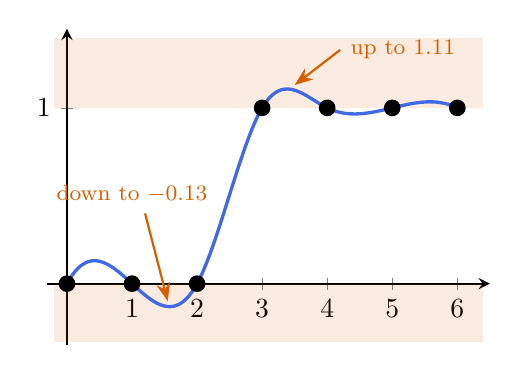
\begin{tikzpicture}
\begin{axis}[width=7.2cm, height=5.6cm, axis lines=middle, xmin=-0.3, xmax=6.5, ymin=-0.35, ymax=1.45,
  xtick={0,...,6}, ytick={1}, thick, clip=false,
  legend style={font=\footnotesize, at={(0.5,1.02)}, anchor=south, draw=none}, legend columns=2]
  \fill[hl, opacity=0.12] (axis cs:-0.2,1) rectangle (axis cs:6.4,1.4);
  \fill[hl, opacity=0.12] (axis cs:-0.2,-0.33) rectangle (axis cs:6.4,0);
  \addplot[accent, very thick] coordinates {(0.0000,0.0000) (0.0250,0.0163) (0.0500,0.0314) (0.0750,0.0453) (0.1000,0.0580) (0.1250,0.0696) (0.1500,0.0800) (0.1750,0.0894) (0.2000,0.0977) (0.2250,0.1050) (0.2500,0.1113) (0.2750,0.1167) (0.3000,0.1211) (0.3250,0.1247) (0.3500,0.1274) (0.3750,0.1292) (0.4000,0.1303) (0.4250,0.1306) (0.4500,0.1302) (0.4750,0.1290) (0.5000,0.1272) (0.5250,0.1248) (0.5500,0.1218) (0.5750,0.1182) (0.6000,0.1140) (0.6250,0.1093) (0.6500,0.1042) (0.6750,0.0986) (0.7000,0.0926) (0.7250,0.0862) (0.7500,0.0795) (0.7750,0.0725) (0.8000,0.0651) (0.8250,0.0576) (0.8500,0.0497) (0.8750,0.0417) (0.9000,0.0336) (0.9250,0.0253) (0.9500,0.0169) (0.9750,0.0085) (1.0000,0.0000) (1.0250,-0.0085) (1.0500,-0.0169) (1.0750,-0.0253) (1.1000,-0.0336) (1.1250,-0.0417) (1.1500,-0.0497) (1.1750,-0.0576) (1.2000,-0.0651) (1.2250,-0.0725) (1.2500,-0.0795) (1.2750,-0.0862) (1.3000,-0.0926) (1.3250,-0.0986) (1.3500,-0.1042) (1.3750,-0.1093) (1.4000,-0.1140) (1.4250,-0.1182) (1.4500,-0.1218) (1.4750,-0.1248) (1.5000,-0.1272) (1.5250,-0.1290) (1.5500,-0.1302) (1.5750,-0.1306) (1.6000,-0.1303) (1.6250,-0.1292) (1.6500,-0.1274) (1.6750,-0.1247) (1.7000,-0.1211) (1.7250,-0.1167) (1.7500,-0.1113) (1.7750,-0.1050) (1.8000,-0.0977) (1.8250,-0.0894) (1.8500,-0.0800) (1.8750,-0.0696) (1.9000,-0.0580) (1.9250,-0.0453) (1.9500,-0.0314) (1.9750,-0.0163) (2.0000,0.0000) (2.0250,0.0176) (2.0500,0.0364) (2.0750,0.0563) (2.1000,0.0773) (2.1250,0.0994) (2.1500,0.1223) (2.1750,0.1462) (2.2000,0.1709) (2.2250,0.1963) (2.2500,0.2224) (2.2750,0.2491) (2.3000,0.2764) (2.3250,0.3041) (2.3500,0.3323) (2.3750,0.3609) (2.4000,0.3897) (2.4250,0.4188) (2.4500,0.4480) (2.4750,0.4773) (2.5000,0.5067) (2.5250,0.5360) (2.5500,0.5652) (2.5750,0.5943) (2.6000,0.6231) (2.6250,0.6517) (2.6500,0.6799) (2.6750,0.7076) (2.7000,0.7349) (2.7250,0.7616) (2.7500,0.7877) (2.7750,0.8131) (2.8000,0.8377) (2.8250,0.8615) (2.8500,0.8845) (2.8750,0.9065) (2.9000,0.9275) (2.9250,0.9474) (2.9500,0.9662) (2.9750,0.9837) (3.0000,1.0000) (3.0250,1.0150) (3.0500,1.0286) (3.0750,1.0410) (3.1000,1.0522) (3.1250,1.0623) (3.1500,1.0711) (3.1750,1.0790) (3.2000,1.0857) (3.2250,1.0915) (3.2500,1.0963) (3.2750,1.1001) (3.3000,1.1031) (3.3250,1.1053) (3.3500,1.1066) (3.3750,1.1072) (3.4000,1.1071) (3.4250,1.1064) (3.4500,1.1050) (3.4750,1.1030) (3.5000,1.1004) (3.5250,1.0974) (3.5500,1.0939) (3.5750,1.0900) (3.6000,1.0857) (3.6250,1.0811) (3.6500,1.0762) (3.6750,1.0710) (3.7000,1.0656) (3.7250,1.0601) (3.7500,1.0544) (3.7750,1.0487) (3.8000,1.0429) (3.8250,1.0371) (3.8500,1.0313) (3.8750,1.0256) (3.9000,1.0201) (3.9250,1.0147) (3.9500,1.0095) (3.9750,1.0046) (4.0000,1.0000) (4.0250,0.9957) (4.0500,0.9917) (4.0750,0.9881) (4.1000,0.9847) (4.1250,0.9817) (4.1500,0.9789) (4.1750,0.9765) (4.2000,0.9743) (4.2250,0.9724) (4.2500,0.9707) (4.2750,0.9693) (4.3000,0.9681) (4.3250,0.9672) (4.3500,0.9665) (4.3750,0.9660) (4.4000,0.9657) (4.4250,0.9656) (4.4500,0.9657) (4.4750,0.9660) (4.5000,0.9665) (4.5250,0.9672) (4.5500,0.9680) (4.5750,0.9689) (4.6000,0.9700) (4.6250,0.9712) (4.6500,0.9726) (4.6750,0.9740) (4.7000,0.9756) (4.7250,0.9773) (4.7500,0.9791) (4.7750,0.9809) (4.8000,0.9829) (4.8250,0.9849) (4.8500,0.9869) (4.8750,0.9890) (4.9000,0.9912) (4.9250,0.9933) (4.9500,0.9955) (4.9750,0.9978) (5.0000,1.0000) (5.0250,1.0022) (5.0500,1.0045) (5.0750,1.0067) (5.1000,1.0088) (5.1250,1.0110) (5.1500,1.0131) (5.1750,1.0151) (5.2000,1.0171) (5.2250,1.0191) (5.2500,1.0209) (5.2750,1.0227) (5.3000,1.0244) (5.3250,1.0260) (5.3500,1.0274) (5.3750,1.0288) (5.4000,1.0300) (5.4250,1.0311) (5.4500,1.0320) (5.4750,1.0328) (5.5000,1.0335) (5.5250,1.0340) (5.5500,1.0343) (5.5750,1.0344) (5.6000,1.0343) (5.6250,1.0340) (5.6500,1.0335) (5.6750,1.0328) (5.7000,1.0319) (5.7250,1.0307) (5.7500,1.0293) (5.7750,1.0276) (5.8000,1.0257) (5.8250,1.0235) (5.8500,1.0211) (5.8750,1.0183) (5.9000,1.0153) (5.9250,1.0119) (5.9500,1.0083) (5.9750,1.0043) (6.0000,1.0000)};
  \addplot[black, only marks, mark=*, mark size=2.6pt] coordinates {(0,0) (1,0) (2,0) (3,1) (4,1) (5,1) (6,1)};
  \draw[hl, thick, -{Stealth}] (axis cs:4.2,1.33) -- (axis cs:3.5,1.13);
  \node[hl, font=\footnotesize, anchor=west] at (axis cs:4.2,1.33) {up to $1.11$};
  \draw[hl, thick, -{Stealth}] (axis cs:1.2,0.4) -- (axis cs:1.55,-0.1);
  \node[hl, font=\footnotesize, anchor=south] at (axis cs:1.0,0.4) {down to $-0.13$};
\end{axis}
\end{tikzpicture}\\[2pt]
\footnotesize The spline leaves the data range $[0,1]$.\\
\textbf{Why:} the slopes are linked, so the jump also tilts its neighbours.
\end{column}
\end{columns}
\end{frame}

% ============================================================
% 6. Shape preserving: the rule
% ============================================================
\begin{frame}{Rule B, shape-preserving (PCHIP): choose slopes locally}
\begin{columns}[c]
\begin{column}{0.46\textwidth}
\small
Look only at the two \textbf{secant slopes} next to node $i$: $\delta_{i-1}$ (left) and $\delta_i$ (right).
\vspace{0.2cm}
\begin{block}{PCHIP rule}
\footnotesize
\textbf{1.} Data turn or go flat (different signs, or a 0)\\
\hspace*{1em}$\Rightarrow d_i = 0$\\[4pt]
\textbf{2.} Otherwise, \textbf{harmonic mean}:
\[
\frac{1}{d_i} = \frac{1}{2}\left(\frac{1}{\delta_{i-1}} + \frac{1}{\delta_i}\right)
\]
\end{block}
\footnotesize
The harmonic mean stays close to the \textbf{smaller} slope, so the curve does not shoot past the data.
\end{column}
\begin{column}{0.52\textwidth}
\centering
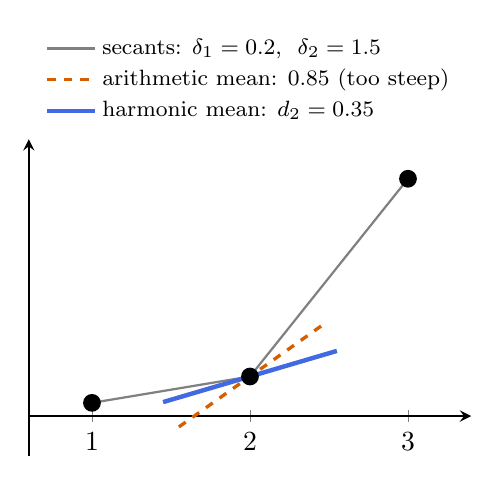
\begin{tikzpicture}
\begin{axis}[width=7.2cm, height=5.6cm, axis lines=middle, xmin=0.6, xmax=3.4, ymin=-0.3, ymax=2.1,
  xtick={1,2,3}, ytick=\empty, thick, clip=false,
  legend style={font=\footnotesize, at={(0.5,1.02)}, anchor=south, draw=none}, legend columns=1]
  \addplot[gray, thick] coordinates {(1,0.1) (2,0.3) (3,1.8)};
  \addlegendentry{secants: $\delta_1 = 0.2$, \ $\delta_2 = 1.5$}
  \addplot[hl, very thick, dashed, domain=1.55:2.45] {0.3+0.85*(x-2)};
  \addlegendentry{arithmetic mean: $0.85$ (too steep)}
  \addplot[accent, ultra thick, domain=1.45:2.55] {0.3+0.353*(x-2)};
  \addlegendentry{harmonic mean: $d_2 = 0.35$}
  \addplot[black, only marks, mark=*, mark size=2.8pt] coordinates {(1,0.1) (2,0.3) (3,1.8)};
\end{axis}
\end{tikzpicture}\\[2pt]
\footnotesize Zoom on nodes 1--3 of the running example.
\end{column}
\end{columns}
\end{frame}

% ============================================================
% 7. Shape preserving: the result
% ============================================================
\begin{frame}{Shape-preserving: the result}
\begin{columns}[c]
\begin{column}{0.46\textwidth}
\small
\begin{exampleblock}{What we gain}
\footnotesize
\textbf{Rising data $\Rightarrow$ rising curve.}\\
No overshoot, no dips below the data.\\
Each slope uses only nearby points (local).
\end{exampleblock}
\begin{alertblock}{What we give up}
\footnotesize
$p''$ may jump at the nodes: only $p$ and $p'$ are continuous.
\end{alertblock}
\vspace{0.1cm}
\footnotesize
\textbf{Akima} is a cousin: a weighted average of $\delta_{i-1}$ and $\delta_i$, also local, also avoids wiggles.\\[4pt]
\textbf{Use when} the data must stay physical: positive, increasing, or bounded.
\end{column}
\begin{column}{0.52\textwidth}
\centering
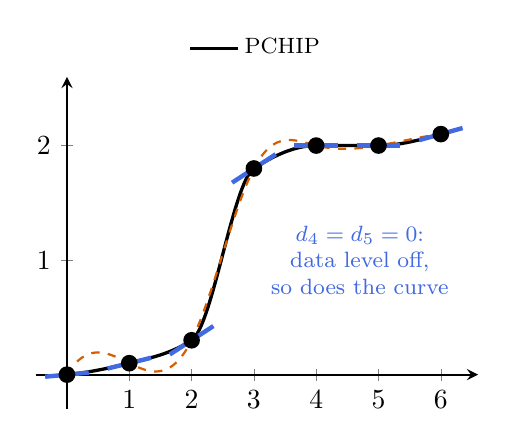
\begin{tikzpicture}
\begin{axis}[width=7.2cm, height=5.8cm, axis lines=middle, xmin=-0.5, xmax=6.6, ymin=-0.3, ymax=2.6,
  xtick={0,...,6}, ytick={1,2}, thick, clip=false,
  legend style={font=\footnotesize, at={(0.5,1.02)}, anchor=south, draw=none}, legend columns=2]
  \addplot[black, very thick] coordinates {(0.0000,0.0000) (0.0250,0.0013) (0.0500,0.0027) (0.0750,0.0041) (0.1000,0.0057) (0.1250,0.0073) (0.1500,0.0089) (0.1750,0.0107) (0.2000,0.0125) (0.2250,0.0144) (0.2500,0.0164) (0.2750,0.0184) (0.3000,0.0206) (0.3250,0.0227) (0.3500,0.0250) (0.3750,0.0272) (0.4000,0.0296) (0.4250,0.0320) (0.4500,0.0345) (0.4750,0.0370) (0.5000,0.0396) (0.5250,0.0422) (0.5500,0.0449) (0.5750,0.0476) (0.6000,0.0504) (0.6250,0.0532) (0.6500,0.0561) (0.6750,0.0590) (0.7000,0.0620) (0.7250,0.0649) (0.7500,0.0680) (0.7750,0.0710) (0.8000,0.0741) (0.8250,0.0773) (0.8500,0.0804) (0.8750,0.0836) (0.9000,0.0869) (0.9250,0.0901) (0.9500,0.0934) (0.9750,0.0967) (1.0000,0.1000) (1.0250,0.1033) (1.0500,0.1066) (1.0750,0.1099) (1.1000,0.1132) (1.1250,0.1165) (1.1500,0.1199) (1.1750,0.1232) (1.2000,0.1266) (1.2250,0.1300) (1.2500,0.1335) (1.2750,0.1370) (1.3000,0.1406) (1.3250,0.1442) (1.3500,0.1480) (1.3750,0.1518) (1.4000,0.1557) (1.4250,0.1597) (1.4500,0.1639) (1.4750,0.1682) (1.5000,0.1725) (1.5250,0.1771) (1.5500,0.1818) (1.5750,0.1866) (1.6000,0.1916) (1.6250,0.1967) (1.6500,0.2021) (1.6750,0.2076) (1.7000,0.2133) (1.7250,0.2192) (1.7500,0.2254) (1.7750,0.2317) (1.8000,0.2383) (1.8250,0.2451) (1.8500,0.2521) (1.8750,0.2595) (1.9000,0.2670) (1.9250,0.2748) (1.9500,0.2829) (1.9750,0.2913) (2.0000,0.3000) (2.0250,0.3109) (2.0500,0.3260) (2.0750,0.3449) (2.1000,0.3674) (2.1250,0.3934) (2.1500,0.4226) (2.1750,0.4549) (2.2000,0.4899) (2.2250,0.5275) (2.2500,0.5675) (2.2750,0.6096) (2.3000,0.6536) (2.3250,0.6994) (2.3500,0.7467) (2.3750,0.7953) (2.4000,0.8449) (2.4250,0.8955) (2.4500,0.9466) (2.4750,0.9982) (2.5000,1.0500) (2.5250,1.1018) (2.5500,1.1534) (2.5750,1.2045) (2.6000,1.2551) (2.6250,1.3047) (2.6500,1.3533) (2.6750,1.4006) (2.7000,1.4464) (2.7250,1.4904) (2.7500,1.5325) (2.7750,1.5725) (2.8000,1.6101) (2.8250,1.6451) (2.8500,1.6774) (2.8750,1.7066) (2.9000,1.7326) (2.9250,1.7551) (2.9500,1.7740) (2.9750,1.7891) (3.0000,1.8000) (3.0250,1.8088) (3.0500,1.8174) (3.0750,1.8259) (3.1000,1.8342) (3.1250,1.8424) (3.1500,1.8504) (3.1750,1.8583) (3.2000,1.8660) (3.2250,1.8735) (3.2500,1.8809) (3.2750,1.8881) (3.3000,1.8951) (3.3250,1.9019) (3.3500,1.9085) (3.3750,1.9150) (3.4000,1.9212) (3.4250,1.9273) (3.4500,1.9331) (3.4750,1.9387) (3.5000,1.9441) (3.5250,1.9493) (3.5500,1.9543) (3.5750,1.9590) (3.6000,1.9635) (3.6250,1.9677) (3.6500,1.9718) (3.6750,1.9755) (3.7000,1.9790) (3.7250,1.9823) (3.7500,1.9853) (3.7750,1.9880) (3.8000,1.9905) (3.8250,1.9927) (3.8500,1.9946) (3.8750,1.9962) (3.9000,1.9976) (3.9250,1.9986) (3.9500,1.9994) (3.9750,1.9998) (4.0000,2.0000) (4.0250,2.0000) (4.0500,2.0000) (4.0750,2.0000) (4.1000,2.0000) (4.1250,2.0000) (4.1500,2.0000) (4.1750,2.0000) (4.2000,2.0000) (4.2250,2.0000) (4.2500,2.0000) (4.2750,2.0000) (4.3000,2.0000) (4.3250,2.0000) (4.3500,2.0000) (4.3750,2.0000) (4.4000,2.0000) (4.4250,2.0000) (4.4500,2.0000) (4.4750,2.0000) (4.5000,2.0000) (4.5250,2.0000) (4.5500,2.0000) (4.5750,2.0000) (4.6000,2.0000) (4.6250,2.0000) (4.6500,2.0000) (4.6750,2.0000) (4.7000,2.0000) (4.7250,2.0000) (4.7500,2.0000) (4.7750,2.0000) (4.8000,2.0000) (4.8250,2.0000) (4.8500,2.0000) (4.8750,2.0000) (4.9000,2.0000) (4.9250,2.0000) (4.9500,2.0000) (4.9750,2.0000) (5.0000,2.0000) (5.0250,2.0001) (5.0500,2.0004) (5.0750,2.0008) (5.1000,2.0015) (5.1250,2.0022) (5.1500,2.0032) (5.1750,2.0043) (5.2000,2.0056) (5.2250,2.0070) (5.2500,2.0086) (5.2750,2.0103) (5.3000,2.0122) (5.3250,2.0141) (5.3500,2.0162) (5.3750,2.0185) (5.4000,2.0208) (5.4250,2.0233) (5.4500,2.0258) (5.4750,2.0285) (5.5000,2.0312) (5.5250,2.0341) (5.5500,2.0371) (5.5750,2.0401) (5.6000,2.0432) (5.6250,2.0464) (5.6500,2.0496) (5.6750,2.0530) (5.7000,2.0564) (5.7250,2.0598) (5.7500,2.0633) (5.7750,2.0668) (5.8000,2.0704) (5.8250,2.0740) (5.8500,2.0777) (5.8750,2.0813) (5.9000,2.0851) (5.9250,2.0888) (5.9500,2.0925) (5.9750,2.0963) (6.0000,2.1000)};
  \addlegendentry{PCHIP}
  \addplot[hl, thick, dashed] coordinates {(0.0000,0.0000) (0.0250,0.0213) (0.0500,0.0412) (0.0750,0.0596) (0.1000,0.0766) (0.1250,0.0924) (0.1500,0.1068) (0.1750,0.1199) (0.2000,0.1318) (0.2250,0.1426) (0.2500,0.1521) (0.2750,0.1606) (0.3000,0.1680) (0.3250,0.1744) (0.3500,0.1798) (0.3750,0.1842) (0.4000,0.1878) (0.4250,0.1904) (0.4500,0.1922) (0.4750,0.1933) (0.5000,0.1935) (0.5250,0.1931) (0.5500,0.1919) (0.5750,0.1902) (0.6000,0.1878) (0.6250,0.1849) (0.6500,0.1814) (0.6750,0.1775) (0.7000,0.1731) (0.7250,0.1683) (0.7500,0.1631) (0.7750,0.1577) (0.8000,0.1519) (0.8250,0.1459) (0.8500,0.1396) (0.8750,0.1332) (0.9000,0.1267) (0.9250,0.1201) (0.9500,0.1134) (0.9750,0.1067) (1.0000,0.1000) (1.0250,0.0934) (1.0500,0.0869) (1.0750,0.0805) (1.1000,0.0743) (1.1250,0.0683) (1.1500,0.0626) (1.1750,0.0572) (1.2000,0.0521) (1.2250,0.0474) (1.2500,0.0431) (1.2750,0.0393) (1.3000,0.0359) (1.3250,0.0331) (1.3500,0.0308) (1.3750,0.0292) (1.4000,0.0282) (1.4250,0.0279) (1.4500,0.0283) (1.4750,0.0295) (1.5000,0.0315) (1.5250,0.0343) (1.5500,0.0380) (1.5750,0.0426) (1.6000,0.0482) (1.6250,0.0548) (1.6500,0.0624) (1.6750,0.0711) (1.7000,0.0810) (1.7250,0.0919) (1.7500,0.1041) (1.7750,0.1175) (1.8000,0.1322) (1.8250,0.1482) (1.8500,0.1655) (1.8750,0.1842) (1.9000,0.2044) (1.9250,0.2260) (1.9500,0.2491) (1.9750,0.2738) (2.0000,0.3000) (2.0250,0.3279) (2.0500,0.3572) (2.0750,0.3881) (2.1000,0.4203) (2.1250,0.4538) (2.1500,0.4886) (2.1750,0.5244) (2.2000,0.5613) (2.2250,0.5992) (2.2500,0.6379) (2.2750,0.6775) (2.3000,0.7177) (2.3250,0.7586) (2.3500,0.8000) (2.3750,0.8419) (2.4000,0.8842) (2.4250,0.9268) (2.4500,0.9696) (2.4750,1.0126) (2.5000,1.0556) (2.5250,1.0986) (2.5500,1.1414) (2.5750,1.1841) (2.6000,1.2265) (2.6250,1.2685) (2.6500,1.3101) (2.6750,1.3512) (2.7000,1.3917) (2.7250,1.4314) (2.7500,1.4705) (2.7750,1.5086) (2.8000,1.5458) (2.8250,1.5820) (2.8500,1.6171) (2.8750,1.6510) (2.9000,1.6837) (2.9250,1.7150) (2.9500,1.7449) (2.9750,1.7732) (3.0000,1.8000) (3.0250,1.8251) (3.0500,1.8486) (3.0750,1.8705) (3.1000,1.8908) (3.1250,1.9097) (3.1500,1.9271) (3.1750,1.9431) (3.2000,1.9578) (3.2250,1.9712) (3.2500,1.9833) (3.2750,1.9943) (3.3000,2.0040) (3.3250,2.0127) (3.3500,2.0203) (3.3750,2.0269) (3.4000,2.0325) (3.4250,2.0372) (3.4500,2.0410) (3.4750,2.0440) (3.5000,2.0462) (3.5250,2.0477) (3.5500,2.0485) (3.5750,2.0487) (3.6000,2.0482) (3.6250,2.0473) (3.6500,2.0458) (3.6750,2.0439) (3.7000,2.0416) (3.7250,2.0389) (3.7500,2.0360) (3.7750,2.0327) (3.8000,2.0293) (3.8250,2.0257) (3.8500,2.0220) (3.8750,2.0182) (3.9000,2.0144) (3.9250,2.0107) (3.9500,2.0070) (3.9750,2.0034) (4.0000,2.0000) (4.0250,1.9968) (4.0500,1.9938) (4.0750,1.9910) (4.1000,1.9885) (4.1250,1.9861) (4.1500,1.9839) (4.1750,1.9820) (4.2000,1.9802) (4.2250,1.9786) (4.2500,1.9771) (4.2750,1.9759) (4.3000,1.9748) (4.3250,1.9739) (4.3500,1.9732) (4.3750,1.9726) (4.4000,1.9722) (4.4250,1.9720) (4.4500,1.9719) (4.4750,1.9719) (4.5000,1.9721) (4.5250,1.9724) (4.5500,1.9729) (4.5750,1.9735) (4.6000,1.9742) (4.6250,1.9750) (4.6500,1.9760) (4.6750,1.9771) (4.7000,1.9783) (4.7250,1.9796) (4.7500,1.9810) (4.7750,1.9825) (4.8000,1.9841) (4.8250,1.9858) (4.8500,1.9876) (4.8750,1.9895) (4.9000,1.9914) (4.9250,1.9935) (4.9500,1.9956) (4.9750,1.9978) (5.0000,2.0000) (5.0250,2.0023) (5.0500,2.0047) (5.0750,2.0071) (5.1000,2.0096) (5.1250,2.0121) (5.1500,2.0146) (5.1750,2.0172) (5.2000,2.0199) (5.2250,2.0226) (5.2500,2.0253) (5.2750,2.0280) (5.3000,2.0307) (5.3250,2.0335) (5.3500,2.0362) (5.3750,2.0390) (5.4000,2.0418) (5.4250,2.0446) (5.4500,2.0474) (5.4750,2.0501) (5.5000,2.0529) (5.5250,2.0557) (5.5500,2.0584) (5.5750,2.0611) (5.6000,2.0638) (5.6250,2.0664) (5.6500,2.0690) (5.6750,2.0716) (5.7000,2.0742) (5.7250,2.0767) (5.7500,2.0791) (5.7750,2.0815) (5.8000,2.0838) (5.8250,2.0861) (5.8500,2.0883) (5.8750,2.0905) (5.9000,2.0925) (5.9250,2.0945) (5.9500,2.0964) (5.9750,2.0983) (6.0000,2.1000)};
  \draw[accent, line width=1.6pt] (axis cs:-0.350,-0.018) -- (axis cs:0.350,0.018); \draw[accent, line width=1.6pt] (axis cs:0.650,0.053) -- (axis cs:1.350,0.147); \draw[accent, line width=1.6pt] (axis cs:1.650,0.176) -- (axis cs:2.350,0.424); \draw[accent, line width=1.6pt] (axis cs:2.650,1.676) -- (axis cs:3.350,1.924); \draw[accent, line width=1.6pt] (axis cs:3.650,2.000) -- (axis cs:4.350,2.000); \draw[accent, line width=1.6pt] (axis cs:4.650,2.000) -- (axis cs:5.350,2.000); \draw[accent, line width=1.6pt] (axis cs:5.650,2.047) -- (axis cs:6.350,2.153);

  \addplot[black, only marks, mark=*, mark size=2.6pt] coordinates {(0.0000,0.0000) (1.0000,0.1000) (2.0000,0.3000) (3.0000,1.8000) (4.0000,2.0000) (5.0000,2.0000) (6.0000,2.1000)};
  \node[accent, font=\footnotesize, align=center] at (axis cs:4.7,1.0) {$d_4 = d_5 = 0$:\\data level off,\\so does the curve};
\end{axis}
\end{tikzpicture}\\[2pt]
\footnotesize PCHIP never goes down and never exceeds 2.1.
\end{column}
\end{columns}
\end{frame}

% ============================================================
% 8. Summary
% ============================================================
\begin{frame}{Summary: how each method decides the curve}
\small
\centering
\setlength{\tabcolsep}{6pt}
\renewcommand{\arraystretch}{1.4}
\begin{tabular}{llll}
\toprule
\textbf{Method} & \textbf{How it is decided} & \textbf{Smooth} & \textbf{Overshoot?} \\
\midrule
Straight lines & 2 neighbouring values & $p$ & never \\
One polynomial & all points at once & all orders & often \\
Cubic spline & slopes from a global system & $p, p', p''$ & sometimes \\
PCHIP / Akima & slopes from nearby secants & $p, p'$ & no / rarely \\
\bottomrule
\end{tabular}
\vspace{0.4cm}
\raggedright
\begin{block}{Take-home messages}
\footnotesize
\begin{enumerate}
  \setlength{\itemsep}{3pt}
  \item The trade-off is \textbf{smoothness vs locality}.
  \item Piecewise cubics differ only in \textbf{how the slopes $d_i$ are chosen}.
  \item Smooth data, smooth curve wanted: \textbf{cubic spline}. Data must keep its shape: \textbf{PCHIP}.
\end{enumerate}
\end{block}
\end{frame}

\end{document}
